\renewcommand{\arraystretch}{1.5}
\chapter[Jake \LILLYxBOXxVersion{\small 1.0.8}]{Jake}
\elable{mrk:JAKE}\TitleSUB{\Jake[]! Would you get me the cake please?\ldots \hfill \LILLYxBOXxVersion{\small 1.0.8}}
\section{Grundlegendes}\elable{jmp:iJake}
\subsection{Entwicklung}
Anfänglich wurde \Jake als \emph{installer} konzipiert, der einfach nur die mühsehlige Installation
des Pakets abnehmen soll. Mittlerweile hat sich \Jake allerdings weiterentwickelt und
bietet das Potenzial für einiges mehr. Im Folgenden sei die Funktionsweise genauer erklärt.
Zu beachten ist allerdings, dass \Jake bisher nur für Linux und MacOS einen Installer und somit
seine Funktionalität zur Verfügung stellt!

\subsection{Die Installation}
\elable{mrk:InstallJake}Jake wird als \T{.jar}-Datei geliefert und lässt sich, eine vorhandene Installation von Java vorrausgesetzt, durch das bloße ausführen installieren. Auf Linux kann dies zum Beispiel wie folgt von statten gehen:
\begin{bash}
java -jar jake.jar
\end{bash}
Nach abgeschlossener Installation sollte das Terminal neu gestartet, oder die Konfigurationsdatei neu geladen werden, um Jake zur Verfüung zu stellen. Das bloße Ausführen von \cbash{jake} sollte nun eine Hilfe anzeigen, die über die jeweiligen Optionen aufklärt. 

\begin{bemerkung}[C++ Jake]
\textit{Bis zur Version \LILLYxBOXxVersion{1.0.9} war Jake in C++ geschrieben jund benötigt deswegen eine andere Installation.}\newline
\Jake zu installieren sollte normalerweise einem Kinderspiel gleichen. Notwendig sind hierfür
auf allen bisher unterstützten Betriebssystemen (Debian-Basiertes Linux und MacOS) ein
\verb|C++14| fähiger \T{gcc}-Compiler und \T{make}.
Anschließend gilt es ins \verb|jake_source|-Verzeichnis zu navigieren.
Es befindet sich hier: \T{Lilly/Jake/jake\_source}.
In diesem Verzeichnis kann man nun \T{make} ausführen. Dies sorgt dafür,
dass nicht nur \T{jake.cpp} zu einer ausführbaren Datei wird, sondern auch,
dass \LJake systemweit zur Verfügung steht (sofern die verwendeten Konsole
bash, zsh oder iTerm ist, bzw. im allgemeinen auf eine der folgenden Dateien
zugreift: \T{.bashrc}, \T{.zshrc}, \T{.bash\_profile}).\newline
Damit gilt \Jake als \emph{installiert}.
\end{bemerkung}


\subsection{Lilly mit Jake installieren}
Mit \LILLYxBOXxVersion{2.0.0} liefert \Jake stets eine Version von Lilly mit, die sich nach einem Update automatisch mit dem nächsten Start von \Jake aktualisiert, sofern sie einmal installiert wurde: \bbash{jake install}. Wird hier eine Frage nach verschiedenen Installationsoptionen gestellt, so siehe bei den \jmark[Entwicklerinformationen]{mrk:jakedevinfo} oder wähle einfach die Intallation der enthaltenen Variante (vermutlich Option $2$). Die automatische Aktualisierung wird durch eine Ausgabe getreu \T{[Die Lilly-Installation wurde aktualisiert.]} ausgegeben. Mithilfe von \bbash{jake GUI} kann Jake auch über die Kommandozeile im Grafischen-Modus gestartet werden, allerdings empfiehlt sich hierfür das Verwenden des Eintrags im Anwendungsmenü. 

\subsection{Jake im Überblick}
Hier werden zuerst die Vorzüge der Kommandozeile präsentiert, da die grafische Variante von Jake noch nicht sinnvoll ausgebaut ist und sich bisher lediglich zum editieren von Konfigurationsdateien eignet.
\paragraph{Kommandoszeile}
Im Regelfall, zur Kompilierung eines Dokuments, genügt es \Jake mit dem jeweiligen Dokument aufzurufen:
\begin{bash*}
jake :lan:Dokumentname.tex:ran:
\end{bash*}
Der Kompilierung können nun eine endlose Reihe an Einstellungen übergeben werden die jeweils mit einem \say{\T{-}} anzuführen sind. Eine boolesche Einstellung kann so bereits umgeschaltet werden. So liefert:
\begin{bash*}
jake dump -debug -debug -debug
\end{bash*}
Für die Einstellung \say{\T{debug}} \emph{true}. Eine \say{normale} Einstellung, welche ein Argument fordert wird durch einen Doppelpunkt beendet:
\begin{bash*}
jake dump -lilly-author: "Sonnenprophet Hamsterbacke"
\end{bash*}
Liefert den entsprechenden Author für \T{lilly-author}. Dies lässt sich auch bei booleschen Ausdrücken, hier mit dem Setzen der Werte \emph{true} und \emph{false} erzeugen. Final gibt es noch Listen, die auch so zugewiesen werden können, allerdings durch das anfügen von \T{+:} auch erweitert werden können. So liefert:
\begin{bash*}
jake dump -lilly-boxes: "DEFAULT" -lilly-boxes+: "ALTERNATE"
\end{bash*}
Den Wert \say{\T{DEFAULT ALTERNATE}} für die Einstellung \T{lilly-boxes}, die Trennung der Elemente (Leerfeld) wird von Jake automatisch erkannt ist aber in der Regel auf Leerfelder normiert.\\
Hier die große (und hoffentlich vollständige) Liste aller möglichen Einstellungen. Ist der Standardwert zu lang, so wird er durch \T{\ldots} gekürzt, wenn er abhängig ist, wird dies in der Bemerkung erklärt. Es gilt zu beachten, dass sich durch Konfigurationsdateien alle Einstellungen modifizieren lassen und somit auch die Standardwerte verändern:{%\renewcommand{\arraystretch}{0.95}
\begin{tabularx}{\linewidth}{t~i~t~^>{\scriptsize}X+}
    \toprule
        \headerrow Bezeichner & Typ & Defaultwert & \normalsize Beschreibung \\
    \midrule
        Version & String & [\ldots] & Aktuelle Version von Jake \\
        \headerrow* file & String & dummy.tex & Datei, um die es gehen soll \\
        answer & String & & Antwort, die, sofern nicht leer, auf alle Fragen die Jake stellt zuerst gegeben wird. Ein setzen auf \say{\T{y}} entspricht der \T{-y}-Option von \T{apt}.\\
        \headerrow* operation & String & help & Was Jake tun soll \\
        debug & Boolean & false & Gibt an, ob Debug ausgegeben werden soll oder nicht \\
        debug-filter & String & .* & Veraltet \\
        path & String & ./ & Pfad zu Lilly \\
        what & String & & Zusatzargument für manche Operationen \\
        install-path & String & \${HOME}/texmf & Ziel Pfad der Installation \\
        gepardrule-path & String & & Pfad für Gepardregeln \\
    \midrule 
        lilly-path & String & \$(dirname\ldots & Pfad zur \T{Lilly.cls} \\
        lilly-out & String & ./\$(BASE\ldots & Ausgabeordner der Tex-Datei? \\
        lilly-in & String & ./ & Input-Pfad für Dateien \\
        lilly-nameprefix & String & & Namenspräfix für Ausgabedatei \\
        lilly-boxes & List & DEFAULT & Boxen für den Kompiliervorgang \\
        lily-modes & String & default & Modi für den Kompiliervorgang \\
        lilly-complete & Boolean & true & Vollständige Dokumentvariante \\
        lilly-complete-name & String & COMPLETE- & Präfix der vollständigen Version \\
        lilly-print-name & String & PRINT- & Präfix der Druckversion \\
        lilly-cleans & List & log aux \ldots & Dateiendungen die von \T{autoclean} gelöscht werden \\
        lilly-autoclean & Boolean & true & Sollen Dateien automatisch gelöscht werden? \\
        lilly-compiletimes & String & 2 & Wie oft soll kompiliert werden \\
        lilly-vorlesung & String & NONE & Um welche Vorlesung handelt es sich? \\
        lilly-semester & String & 0 & Das wievielte Semester ist es \\
        lilly-n & String & 42 & Um das wievielte Übungsblatt handelt es sich? \\
        lilly-show-boxname & Boolean & true & Soll der Boxname angezeigt werden? \\
        lilly-layout-loader & String & & Pfad zu den Layouts \\
        lilly-external & Boolean & false & Soll versucht werden, Grafiken auszulagern? \\
        lilly-external-out & String & extimg & Ausgabeordner für ausgelagert Grafiken \\
        \headerrow* lilly-author & String & Florian\ldots & Author des Dokuments \\
        \headerrow* lilly-author-mail & String & florian.s\ldots & Email-Adresse des Authors \\
        lilly-signatur-farbe & String & Leaf & Farbe für das Highlighting \\
        lilly-bibtex & String & & Bibtex-Datei (ohne Endung) \\
        lilly-doctype & String & Mitschrieb & Typ des Dokuments \\
        lilly-autoconf & Boolean & false & Soll automatisch eine \T{.conf}-Datei gewählt werden? \\
        lilly-configs-path & String & & Pfad zur Lilly-Konfigurationsdatei (\blankcmd{lillyPathConfig})\\
        lilly-data-path & String & & Pfad zu generellen Daten (\blankcmd{lillyPathData})\\
        \midrule
        jobcount & String & 2 & Wie viele verschiedene Threads sollen im multithreaded-compile gleichzeitig betrieben weren? \\
        error-count & String & 5 & Wie viele Fehler sollen in der Vorschau maximal angezeigt werden? \\
        mk-name & String & Makefile & Veraltet, Name des Makefiles \\
        mk-path & String & ./ & Veraltet, Pfad des Makefiles \\
        mk-use & Boolean & false & Veraltet, soll das Makefile verwendet werden? \\
    \bottomrule
\end{tabularx}
}
Zusätzlich kann anstelle der vorangestellten Option wie \T{dump} beziehungsweise der \T{.tex}-Datei auch eine Konfigurationsdatei angegeben werden. Auf sie wird \jmark[hier]{mrk:configfile} % todo: link
mehr eingegangen. Bei einer solchen Angabe handelt es sich um eine Kurzform der jeweiligen Optionen \T{config} und \T{file\_compile}. Ausführlich würde man also zum Kompilieren dieser Dokumentation schreiben:
\begin{bash*}
jake file_compile -file: Lilly-Dokumentation.doc.tex
\end{bash*}
beziehungsweise, zum Verwenden der beiliegenden Konfigurationsdatei:
\begin{bash*}
jake config -file: doc.conf
\end{bash*}
Oder eben die Kurzform:
\begin{bash*}
jake doc.conf
\end{bash*}
Die automatisch die Optionen entsprechend setzt.\smallskip\newline
Als letzte wichtige Funktion sei noch \T{get} genannt, welche für das Paket \LILLYxNOTExLibrary{LILLYxGRAPHICSxPROVIDER} aus \LILLYxNOTExLibrary{LILLYxGRAPHICS} relevant ist. So liefert der Befehl:
\begin{bash}
jake get
\end{bash}
Eine PDF wie die folgende, die alle mit Lilly gelieferten Grafiken enthält:
\begin{tcbraster}[raster columns=3, blankest, graphics pages={13,33,34},colback=white]
    \tcbincludepdf{\LILLYxPATHxDATA/Graphics/all-OUT/all.pdf}
\end{tcbraster}
Angezeigt wurden hier übrigens die Seiten $13$, $33$ und $34$ zum Kompilierzeitpunkt dieser Dokumentation.
\paragraph{Gui}
Wie bereits angemerkt, ist die GUI von \Jake noch nicht ansatzweise ausgereift. Der sich öffnende Hauptdialog erlaubt das Auswählen einer Latex- oder Konfigurationsdatei und zeigt die aus der Datei extrahierten Informationen inklusiver ihrer (sofern verschieden) extrahierten Werte an:
\begin{center}
    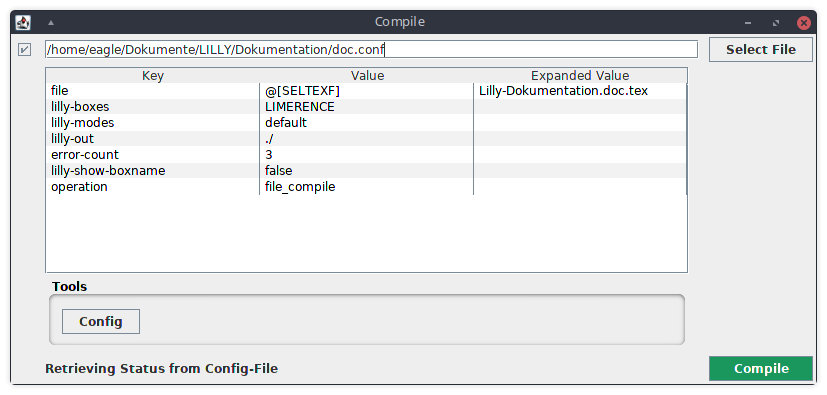
\includegraphics[width=0.75\linewidth]{Data/Bilder/JakeGUIMain.png}
\end{center}
Nebst einem schönen Ausblick auf das was in der GUI-Welt noch so alles geschehen mag, bietet sich der Button \T{Config} an, der im Falle keine ausgewählten Konfigurationsdatei einfach auf einer neuen arbeitet:
\begin{center}
    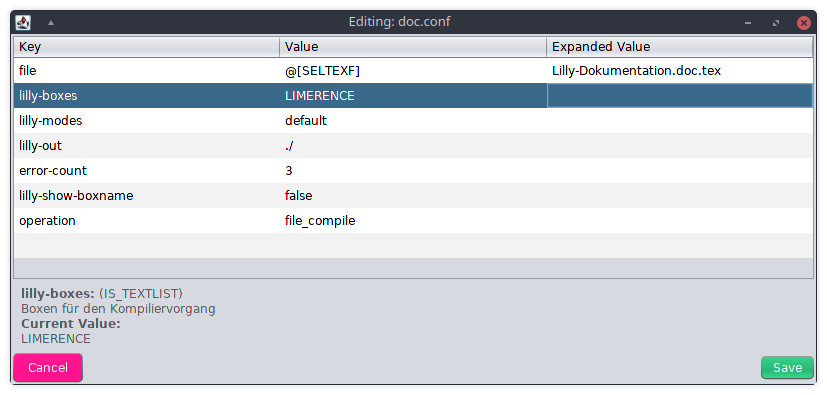
\includegraphics[width=0.5\linewidth]{Data/Bilder/JakeGUIConfig.png}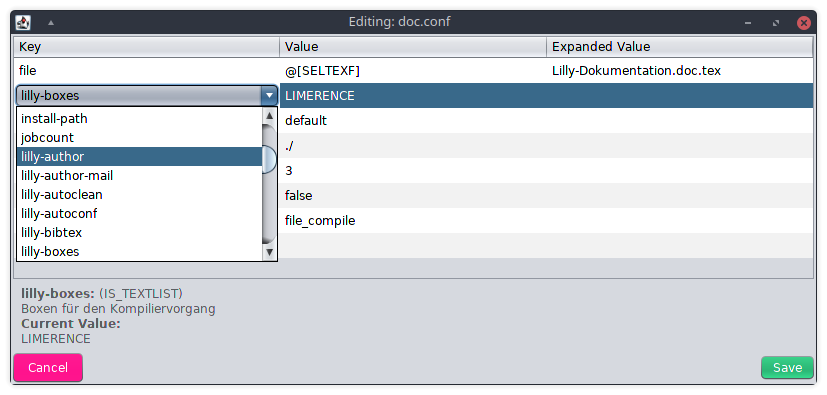
\includegraphics[width=0.5\linewidth]{Data/Bilder/JakeGUIConfigSelection.png}    
\end{center}
Hier werden nicht nur einige Informationen zu den jeweileigen Einstellungen angezeigt, sondern auch Plausibilitätsprüfungen durchgeführt. Im Falle einer neuen Konfigurationsdatei kann beim Speichern ein entsprechendes Ziel ausgewählt werden. 

\subsection{Entwicklerinformationen}
\elable{mrk:jakedevinfo}% Note that update will occur even if lilly hasn't updated, but jake has. 
